

\section{ApoCo Use Cases}

\subsection{Use Case- Diagramm}

Die Abbildung 4.11 veranschaulicht ein Use Case-Diagramm der ApoCo-Anwendung.
Hier werden Interaktionsm\"oglichkeiten des Benutzers mit der Android-Anwendung und die Kommunikation 
mit dem Webserver abgebildet.
\begin{figure}[h]
  \centering
  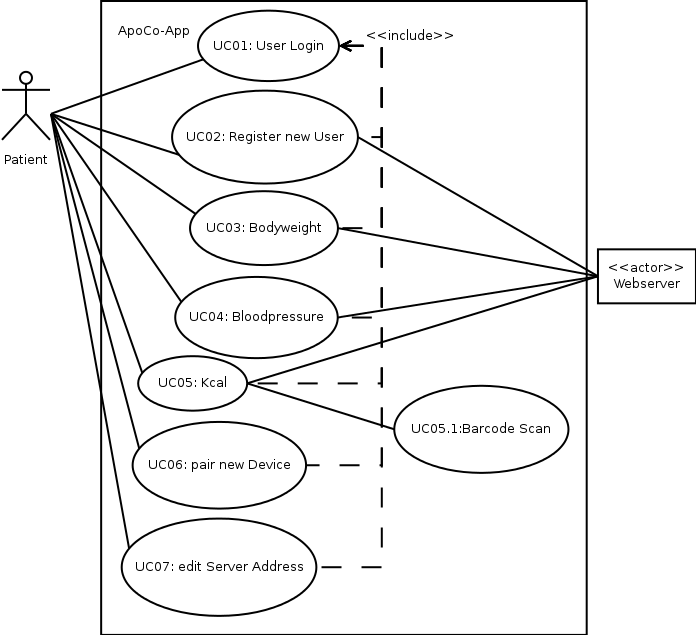
\includegraphics[scale=0.6]{diagramme/kapitel4/use_cases.png}
  \caption{ApoCo Use Case-Diagramm}
  
\end{figure}

\subsection{Aktoren}

\begin{itemize}
 \item Patient: Benutzer der ApoCo-Anwendung
 \item Webserver: Webserver mit Service zur Verwaltung der Tagesprotokolle
\end{itemize}

\subsection{Use Case Kurzbeschreibungen}

\begin{itemize}
 \item UC01: User Login\\ 
 Der Benutzer Meldet sich bei der ApoCo-Anwendung an.
 \item UC02: Register new User\\ 
 Ein neuer Benutzer registriert sich im System.
 Die Benutzerdaten werden zum Server gesendet und von diesem erlaubt oder verweigert.
 \item UC03: Bodyweight\\ 
 Der Benutzer f\"uhrt eine K\"orpergewichtsmessung durch.
 Zielgewicht wird vom Server geladen.
 Die Messung wird an den Server gesendet.
 \item UC04: Bloodpressure\\ 
 Der Benutzer f\"uhrt eine Blutdruckmessung durch.
 Die Messung wird an den Server gesendet.
 \item UC05: Kcal\\ 
 Der Benutzer f\"uhrt eine Protokollierung seiner Mahlzeit durch.
 Informationen zum Lebensmittel werden vom Webserver geladen.
 Mahlzeitprotokoll wird an den Server gesendet.
 \item UC05.1: Barcode Scan\\ 
 Der Benutzer scannt w\"ahrend einer Mahlzeitprotokollierung ein Lebensmittel mittels Barcodescanner ein.
 \item UC06: Pair new Device\\ 
 Der Benutzer f\"uhrt eine Ger\"ate-Koppelung durch.
 \item UC07: edit Server Address\\ 
 Der Benutzer konfiguriert die Webadresse des Servers.
\end{itemize} 
